\section{A Framework for Scalability Testing}

The Scalability Testing Framework aims at assisting the scalability explorer, the person who tests the scalability, to verify the scalability of an application. Based on the research presented in the last section, we conclude that the tester must apply the following steps to assess a system scalability. 

\begin{enumerate}
\item Choose the variables of the problem complexity, the performance, and the architecture;
\item Define the functions of the complexity size of the problem, performance metric, and the architecture capability;
\item Choose initial values for these variables;
\item Execute the application with these initial values for obtaining the initial value of the performance metric;
\item Execute multiple times with the same process and collect the performance metric for each execution;
\item Analyze the performance metric.
\end{enumerate}

For the reason that we do not want to restrict which type of scalability the tester will make, we choose to develop a framework where steps 1 to 3 could be made without limitations.
To support the scalability explorer, the Scalability Testing Framework automates the steps 4 and 5, which are repetitive process. It, also, assists the analysis of the performance metric obtained (Step 6).

It has been developed in Java and it may be used with it or with languages that run on the JVM (Java Virtual Machine) and can be used with Java Annotations, such as Scala.

The scalability explorer needs to execute the same process multiple times by only changing the variables that define the complexity size of the problem and the architecture capability. To support that, the framework provides two Java Annotations \emph{@ScalabilityTest} and \emph{@Scale} that gives the ability to the scalability explorer to execute steps 4 and 5. The tester must only specify one method that describes the execution and the variables that need to change for each execution.

\lstset{caption={Scalability test method template},label=MethodTemplate}
\begin{lstlisting}
@ScalabilityTest(scalabilityFunction=<ScalabilityFunction.class>, steps=<Integer>)
public List<Number> methodName(@Scale Number parameterScale, Object parameter) {
	//execution process
	return performanceMetrics;
}

\end{lstlisting}

A template of the method that is executed by the framework is shown in snippet \ref{MethodTemplate}. The annotation \emph{@ScalabilityTest} has two parameters: \emph{scalabilityFunction} and \emph{steps}. The \emph{steps} parameter defines how many times the method will be executed, we call each execution as a \emph{step}.

With the \emph{scalabilityFunction} parameter, the scalability explorer specifies how the method parameters with the annotation \emph{@Scale} will increase for each step. The parameter specified is a class that extends the ScalabilityFunction class. The classes available are \emph{LinearIncrease}, \emph{ExponentialIncrease}, and \emph{QuadraticIncrease}, which are described with more details below.

The framework collects the performance metric of each step as a list of values. After each execution, it calculates the mean and the standard deviation of these lists to plot them in a graph.

\subsection{Example}

Supposed that we developed a web service which is located in a cloud environment and we want to verify its \emph{load scalability}. Therefore, we choose the number of requests per second to be the complexity size of the problem function, the number of nodes which the web service is running upon as an architecture capability, and the average response time as the performance metric. Code \ref{TestExample} shows an example of scalability test in this case.
\lstset{caption={Scalability test example},label=TestExample}
\begin{lstlisting}
@ScalabilityTest(scalabilityFunction=LinearIncrease.class, steps=5)
public List<Long> scalabilityTest(@Scale int requests, @Scale int numberNodes) {
	List<Long> resposeTimes = new List<Long>();
	instatiateNumberOfNodes(numberNodes); // Change the number of nodes
	responseTimes = makeRequestsPerSecond(requests);//Returns a list of response times
	return responseTimes;
}
\end{lstlisting}

At Line 1 is described that this method is a scalability test which must be execute 5 times  and that the parameters with the \emph{@Scale} annotation(Line 2) should increase linearly. 

At Line 4, we call a method that will change the number of nodes where the web service is deployed. If we increase the number of nodes, we improve the architecture capability. Then, at Line 5, we call a function that makes a number of requests per second to the web service and returns the response times of each execution.

The framework will execute the scalability test with the call presented in the Code \ref{ScalabilityTestCall}. The object \emph{wsScalabilityTest} is the one where the test is described, the string \emph{"scalabilityTest"} is the name of the scalability test, and the integers \emph{1000} and \emph{1} are the initial values of the test parameters.
\lstset{caption={Scalability test call},label=ScalabilityTestCall}
\begin{lstlisting}
ScalabilityReport report;
report = ScalabilityTesting.run(wsScalabilityTest, "scalabilityTest", 1000, 1);
\end{lstlisting}


\begin{figure}[h]
\begin{center}
	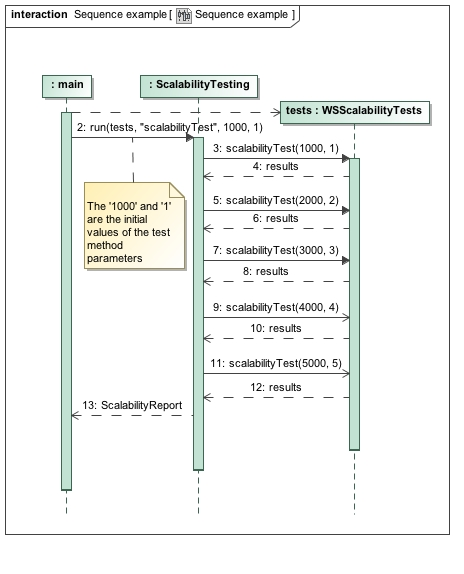
\includegraphics[scale=0.7]{images/sequenceExample.jpg}
\caption{Sequence Diagram of the Example \ref{ScalabilityTestCall}}
\label{sequenceDiagramExample}
\end{center}
\end{figure}

The Sequence Diagram \ref{sequenceDiagramExample} shows the how the example above will be executed by the framework. It will execute 5 times, increasing the test parameters linearly, collecting the results, and calculating the mean and the standard deviation for each execution step. After the execution, the framework returns a \emph{ScalabilityReport} object where contains the information about the execution.

Code \ref{GraphPlotExample} shows how to use the report to plot a graph using the \emph{ScalabilityReportChart}. Since it can plot more than one scalability test for comparisons, it receives a list of reports. The scalability explorer can also specify the label for the performance metric axis, which is by default \emph{"Performance metric"}. Image \ref{graphIllustration} shows a graph illustration of the example above.

\lstset{caption={Graph plotting code example},label=GraphPlotExample}
\begin{lstlisting}
ScalabilityReportChart chart = new ScalabilityReportChart();
List<ScalabilityReport> reports = new ArrayList<ScalabilityReport>();
reports.add(report);
chart.createChart(reports, "average response time (ms)");
\end{lstlisting}

\begin{figure}[t]
\begin{center}
	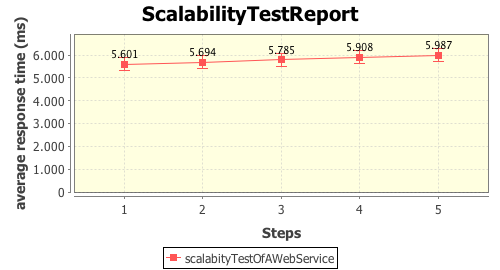
\includegraphics[scale=0.7]{images/graphExample}
\caption{Graph Illustration}
\label{graphIllustration}
\end{center}
\end{figure}

\subsection{Architecture}
The Scalability Testing Framework is composed by three main packages, one related to the framework hot spots, where the annotations is located, one used to interpret the annotations and execute the scalability tests, and another to show the scalability testing report to the scalability explorer. The class diagram is presented in Figure \ref{classDiagram}.

\begin{figure}[htbp]
\begin{center}
	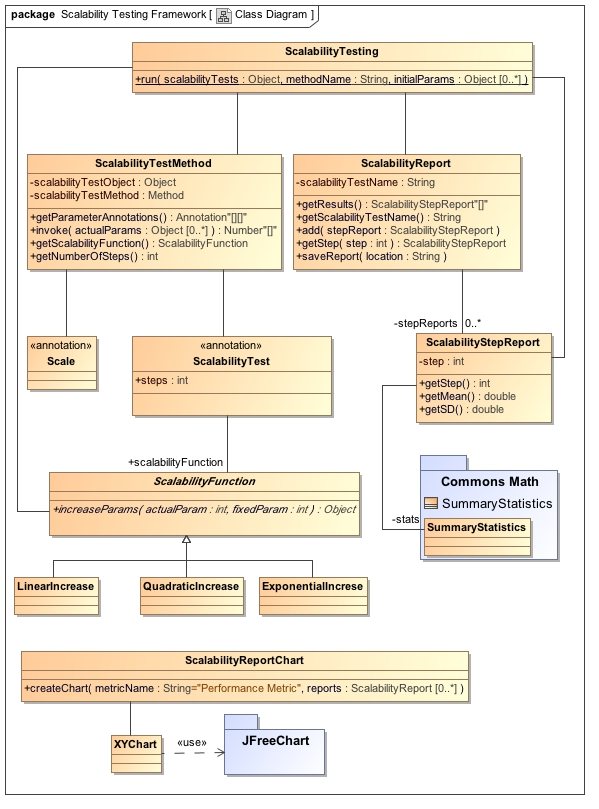
\includegraphics[scale=0.75]{images/classDiagram.jpg}
\caption{Scalability Testing Framework Class Diagram}
\label{classDiagram}
\end{center}
\end{figure}

\subsubsection{Framework Hot Spots: Annotations and Scalability Increase Functions}
The Scalability Testing Framework has two principal hot spots. A hot spot of a framework is a place of the architecture where the developer can add and modified desired functionalities to adapt the application. In this case, for instance, the test specification is a content that the tester will add to execute the framework. The firsts hot spots the framework provides are the two Java Annotations, \emph{@ScalabilityTest} and \emph{@Scale}.

The \emph{@Scale} annotation is a parameter annotation. It must be located before the specification of the parameter and the parameter type. The parameters with this annotation will be increased by the framework in each execution step.

The \emph{@ScalabilityTest} annotation is a method annotation, which means that it must be used for methods and it is located right above the method that describes a scalability test. It has two parameters. The \emph{steps} describes how many steps the framework will make to execute the test. The \emph{scalabilityFunction} describes how the method parameters with the \emph{@Scale} will increase in each step. It is defined by a class that extends the \emph{ScalabilityFunction} class.

This is the second principal hot spot of the framework. There are, already, three ScalabilityFunction class implemented:
\begin{description}
\item[LinearIncrease] increases the parameters linearly. Thus, a parameter with initial value $x$ will be $2x$ in the second step and $nx$ in step $n$.
\item[ExponetialIncrease] increases the parameters exponentially. The parameter with initial value $x$ will be $x \times 2$ in the second step and $x \times 2^n$ in step $n$.
\item[QuadraticIncrease] increases the parameters quadratically. The parameter with initial value $x$ will be $x \times 2^2$ in the second step and $x \times n^2$ in step $n$.
\end{description}

However, the scalability explorer can develop other scalability function for a particular case if needed. The class must extend the \emph{ScalabilityFunction} class which has a method that defines how a parameter will increase. It receives two integers with the last value used and the initial value and must return a new value.

\subsubsection{ScalabilityTests Interpreters}
The \emph{ScalabilityTesting} class is called by the scalability explorer to execute the scalability tests. It executes the scalability test based on the parameters specified in the annotations \emph{@ScalabilityTest} and \emph{@Scale}. It uses the \emph{ScalabilityTestMethod} class, that interprets the annotations of the scalability tests, to collect information of them.

For each step, a \emph{ScalabilityStepReport} is instantiated with the results. With the support of the Commons Math package, it calculates the mean and the stardard deviation of the performance metrics.

After the execution, the \emph{ScalabilityTesting} class instantiates a \emph{ScalabilityReport} that has a list of \emph{ScalaiblityStepReport}. This class can be used by the scalability explorer to a plot a graph to analyze the results.

\subsubsection{Scalability Tests Graph}
The scalability explorer can plot the result of one or more scalability tests with their \emph{ScalabilityReport} using the \emph{ScalabilityReportChart}. This class uses the \emph{XYChart} class, that has the procedure to plot the graph with the support of the JFreeChart package.


\subsection{Implementation}

The framework was developed in Java since it belongs to the Rehearsal Framework, which is in Java. We've been developed it using Test-Driven Development (TDD), described in the introduction, with the support of the JUnit Framework\footnote{http://www.junit.org/} to specify and run the tests.

The development has been done using the Eclipse IDE\footnote{http://www.eclipse.org/} with the support of the plugins EclEmma\footnote{http://www.eclemma.org/} and Eclipse Metrics\footnote{http://eclipse-metrics.sourceforge.net/}. The first one is a Java code coverage tool to verify the coverage of the tests in the code. The Scalability Testing Framework has 100\% of test coverage. The second one calculates some metrics of the code, such as cohesion metrics, which made us developed a code with quality.\\

The Scalability Testing Framework uses two third-partner libraries:
\begin{description}
\item[JFreeChart\footnote{http://www.jfree.org/jfreechart/}] to plot the performance metric graphs. It is depends on the JCommon library. Both are licensed under the terms of GNU Lesser General Public License (LGPL). 
\item[Math Commons\footnote{http://commons.apache.org/math/}] to calculate statistical values of the performance values returned by the scalability tests. It is licensed under the terms of Apache License.
\end{description}

The project used the Design Pattern Strategy[\citet{GOF1995}] in the implementation of the functionality that increases the parameters in each step. The Strategy structure is presented in Figure \ref{strategyStructure}. 

The \emph{ScalabilityTesting} class, that executes the tests, collects a \emph{ScalabilityFunction} class, the strategy class, and increases the test parameters without the knowledge of which strategy is being used. The concrete strategy classes can be the \emph{LinearIncrease}, \emph{ExponentialIncrease}, \emph{QuadraticIncrease}, and another class developed by the scalability explorer that extends the \emph{ScalabilityFunciton} class. As we can observe in Figure \ref{classDiagram}, the structure of the classes described is equivalent to the Strategy Structure.
\begin{figure}[htbp]
\begin{center}
	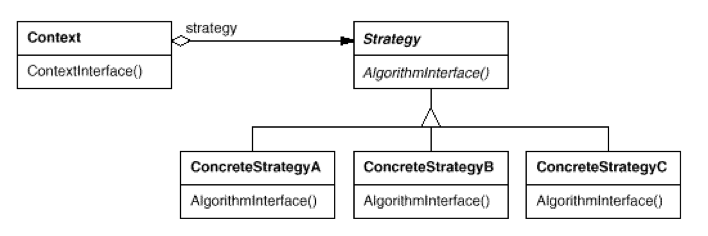
\includegraphics[scale=0.5]{images/strategyStructure}
\caption{Design Pattern Strategy Structure from \citet{GOF1995}}
\label{strategyStructure}
\end{center}
\end{figure}


